\documentclass[12pt,a4paper]{article}
\usepackage[utf8]{vietnam}
\usepackage{amsmath,amssymb}
\usepackage{tabularx}
\usepackage{tikz}
\usetikzlibrary{calc,angles,quotes,arrows.meta,patterns}
\usepackage{xcolor}
\usepackage{enumitem}
\usepackage{fancyhdr}
\usepackage{graphicx}
\usepackage[top=1.0cm, bottom=1.0cm, left=1.2cm, right=1.2cm]{geometry}
\usepackage[dethi]{ex_test}
\SAOPTN{widthSA=3.2,heightSA=0.62}

\setlength{\headheight}{15pt}
\setlength{\parskip}{0pt}

\pagestyle{fancy}
\fancyhf{}
\rhead{\textit{Môn Toán 8 -- Đề số 06}}
\lhead{\textit{Bộ đề ôn tập Giữa học kì I}}
\cfoot{\thepage}

\begin{document}

% --- KHUNG TIÊU ĐỀ ĐỀ THI ---
\noindent
\begin{tabularx}{\linewidth}{X r}
\textbf{TRƯỜNG THCS: \dotfill} & \textbf{ĐỀ KIỂM TRA ĐỊNH KỲ GIỮA HỌC KỲ I} \\
\textbf{Họ và tên: \dotfill} & \textbf{NĂM HỌC 2026 -- 2027} \\
\textbf{Lớp: \dotfill \quad SBD: \dotfill} & \textbf{Môn: TOÁN 8} \\
\hline
\end{tabularx}
\vspace{2mm}

\begin{center}
  \textbf{\large ĐỀ ÔN TẬP GIỮA HỌC KỲ I -- ĐỀ SỐ 06}\\
  \textit{Thời gian làm bài: 90 phút (Không kể thời gian phát đề)}
\end{center}
\vspace{1mm}

% --- PHẦN I ---
\noindent\textbf{\large PHẦN I. CÂU TRẮC NGHIỆM NHIỀU PHƯƠNG ÁN LỰA CHỌN (3,0 điểm)}

\textit{Thí sinh trả lời từ câu 1 đến câu 12. Mỗi câu hỏi thí sinh chỉ chọn một phương án duy nhất.}

\vspace{1mm}
\begin{ex}
Đơn thức $-36a^2b^2x^2y^2$ (với $a, b$ là các hằng số) có hệ số là:
\choice
{\True $-36a^2b^2$}
{$-36$}
{$36a^2b^2$}
{$36a^2$}
\end{ex}

\begin{ex}
Đơn thức nào sau đây đồng dạng với đơn thức $-3x^2y$?
\choice
{$3x^2yz$}
{$xy^2$}
{\True $\dfrac{1}{2}xyx$}
{$-3x^2z$}
\end{ex}

\begin{ex}
Tích của đơn thức $6xy$ và đa thức $2x^2 - 3y$ là đa thức:
\choice
{$12x^3y + 18xy^2$}
{\True $12x^3y - 18xy^2$}
{$12x^2y + 18xy^2$}
{$12x^2y - 18xy^2$}
\end{ex}

\begin{ex}
Điều kiện của số tự nhiên $n$ để phép chia $(4x^{10}y - xy^7 + x^5y^4) : 2x^n y^n$ là phép chia hết:
\choice
{$n = 0$}
{\True $n \in \{0; 1\}$}
{$n = 1$}
{$n = 5$}
\end{ex}

\begin{ex}
Hình bình hành cần có thêm điều kiện nào sau đây thì trở thành hình chữ nhật?
\choice
{\True Có một góc vuông}
{Có hai cạnh kề bằng nhau}
{Có hai đường chéo vuông góc}
{Có hai đường chéo cắt nhau tại trung điểm mỗi đường}
\end{ex}

\begin{ex}
Tích của hai đơn thức $7x^2y$ và $(-xy)$ bằng:
\choice
{\True $-7x^3y^2$}
{$7x^3y^2$}
{$-7x^2y$}
{$6x^3y^2$}
\end{ex}

\begin{ex}
Kết quả thu gọn của biểu thức $(x + 3)^2 - (x - 3)^2$ là:
\choice
{$0$}
{$18$}
{$12x + 18$}
{\True $12x$}
\end{ex}

\begin{ex}
Cho hình vẽ sau, trung đoạn của hình chóp tứ giác đều $S.ABCD$ là đoạn thẳng:
\begin{center}
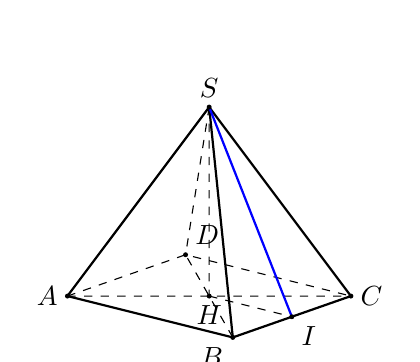
\begin{tikzpicture}[scale=0.75, >=stealth]
  \coordinate (A) at (0,0);
  \coordinate (B) at (2.8,-0.7);
  \coordinate (C) at (4.8,0);
  \coordinate (D) at (2,0.7);
  \coordinate (H) at ($(A)!0.5!(C)$);
  \coordinate (S) at ($(H)+(0,3.2)$);
  \coordinate (I) at ($(B)!0.5!(C)$);
  \draw[dashed] (A)--(D)--(C);
  \draw[dashed] (S)--(D);
  \draw[dashed] (A)--(C) (B)--(D);
  \draw[dashed] (S)--(H);
  \draw[dashed] (H)--(I);
  \draw[thick] (S)--(A)--(B)--(C)--(S);
  \draw[thick] (S)--(B);
  \draw[thick, blue] (S)--(I);
  \fill (A) circle (1.2pt) node[left] {$A$};
  \fill (B) circle (1.2pt) node[below left] {$B$};
  \fill (C) circle (1.2pt) node[right] {$C$};
  \fill (D) circle (1.2pt) node[above right] {$D$};
  \fill (S) circle (1.2pt) node[above] {$S$};
  \fill (H) circle (1.2pt) node[below] {$H$};
  \fill (I) circle (1.2pt) node[below right] {$I$};
\end{tikzpicture}
\end{center}
\choice
{\True $SI$}
{$SA$}
{$SH$}
{$HI$}
\end{ex}

\begin{ex}
Hình chóp tứ giác đều có mặt đáy là hình gì?
\choice
{Tam giác đều}
{Hình chữ nhật}
{\True Hình vuông}
{Hình thoi}
\end{ex}

\begin{ex}
Tứ giác là hình bình hành nếu:
\choice
{Tứ giác có hai góc kề một cạnh bằng nhau}
{Tứ giác có hai cạnh kề bằng nhau}
{\True Tứ giác có các cạnh đối bằng nhau}
{Tứ giác có hai đường chéo bằng nhau}
\end{ex}

\begin{ex}
Khẳng định nào sau đây là đúng?
\choice
{Tứ giác có hai đường chéo vuông góc với nhau là hình bình hành}
{Tứ giác có hai đường chéo bằng nhau là hình thang cân}
{\True Tứ giác có hai đường chéo cắt nhau tại trung điểm mỗi đường là hình bình hành}
{Hình thang có hai cạnh bằng nhau là hình thang cân}
\end{ex}

\begin{ex}
Cho tam giác $ABC$ vuông tại $A$ có $AB = 6\text{ cm}, AC = 8\text{ cm}$. Bán kính đường tròn ngoại tiếp tam giác $ABC$ bằng:
\choice
{$10\text{ cm}$}
{$14\text{ cm}$}
{\True $5\text{ cm}$}
{$7\text{ cm}$}
\end{ex}


\vspace{1mm}
\noindent\textbf{BẢNG TRẢ LỜI TRẮC NGHIỆM PHẦN I:}
\begin{center}
\begin{tabular}{|c|c|c|c|c|c|c|c|c|c|c|c|c|}
\hline
\textbf{Câu} & \textbf{1} & \textbf{2} & \textbf{3} & \textbf{4} & \textbf{5} & \textbf{6} & \textbf{7} & \textbf{8} & \textbf{9} & \textbf{10} & \textbf{11} & \textbf{12} \\
\hline
\textbf{Chọn} & \rule{0pt}{0.65cm} & & & & & & & & & & & \\
\hline
\end{tabular}
\end{center}
\vspace{2mm}

\setcounter{ex}{0}
\noindent\textbf{\large PHẦN II. CÂU TRẮC NGHIỆM ĐÚNG SAI (2,0 điểm)}

\textit{Thí sinh trả lời câu 1 và câu 2. Trong mỗi ý a), b), c), d) ở mỗi câu, thí sinh chọn đúng hoặc sai.}

\vspace{1mm}
\begin{ex}
Cho biểu thức $A = \dfrac{x^2 - 4x + 4}{x - 2} + \dfrac{x^2 - 9}{x + 3}$ với $x \neq 2$ và $x \neq -3$. Xét tính đúng sai của các mệnh đề sau:
\choiceTF
{\True Biến đổi $x^2 - 4x + 4$ thành bình phương của một hiệu ta được $(x - 2)^2$}
{Kết quả rút gọn phân thức $\dfrac{x^2 - 9}{x + 3}$ là $x + 3$}
{\True Kết quả rút gọn của biểu thức $A$ là $2x - 5$}
{\True Tại $x = 4$, giá trị của biểu thức $A$ bằng $3$}
\end{ex}

\begin{ex}
Cho hình bình hành $ABCD$ có $AB = 2AD$. Gọi $M, N$ lần lượt là trung điểm của $AB$ và $CD$. Xét tính đúng sai của các mệnh đề sau:
\choiceTF
{\True Tứ giác $AMCN$ là hình bình hành}
{\True Tứ giác $AMND$ là hình thoi}
{\True Đoạn thẳng $AN$ vuông góc với đoạn thẳng $DM$}
{Cho $\widehat{A} = 60^\circ$, số đo góc $\widehat{AMD}$ bằng $120^\circ$}
\end{ex}


\noindent\textbf{BẢNG TRẢ LỜI PHẦN II:}
\begin{center}
\begin{tabular}{|c|c|c|c|c||c|c|c|c|c|}
\hline
\textbf{Câu 1} & \textbf{a)} & \textbf{b)} & \textbf{c)} & \textbf{d)} & \textbf{Câu 2} & \textbf{a)} & \textbf{b)} & \textbf{c)} & \textbf{d)} \\
\hline
\textbf{Đ/S} & \rule{0pt}{0.6cm} & & & & \textbf{Đ/S} & & & & \\
\hline
\end{tabular}
\end{center}
\vspace{2mm}

\setcounter{ex}{0}
\noindent\textbf{\large PHẦN III. CÂU HỎI TRẢ LỜI NGẮN (2,0 điểm)}

\textit{Thí sinh trả lời câu 1 và câu 2. Điền kết quả vào ô trống tương ứng.}

\vspace{1mm}
\begin{ex}
Tìm $x$, biết: $2x(x - 5) - x + 5 = 0$. \shortans{$x = 5$ hoặc $x = \dfrac{1}{2}$}
\end{ex}

\begin{ex}
Cho hình chữ nhật $ABCD$ có $AB = 8\text{ cm}$ và $BC = 6\text{ cm}$. Tính độ dài đường chéo $AC$. \shortans{$10\text{ cm}$}
\end{ex}


\setcounter{ex}{0}
\noindent\textbf{\large PHẦN IV. TỰ LUẬN (3,0 điểm)}

\textit{Thí sinh trình bày chi tiết lời giải vào giấy làm bài.}

\vspace{1mm}
\begin{ex} (1,0 điểm)
Thực hiện phép tính:
\begin{enumerate}[label=\textbf{\alph*)}, leftmargin=0.8cm, itemsep=2pt]
\item (0,5 điểm) $xy(x^2 - 5xy^2)$
\item (0,5 điểm) $(12x^4y^3 - 5x^3y^2 + 9x^2y^2) : (-3x^2y^2)$
\end{enumerate}
\end{ex}
\vspace{0.5mm}

\begin{ex} (0,75 điểm)
Cho hai đa thức: $M = xy - 3x^2y^2 + x^4 - 5y^3$ và $N = x^4 - 5y^3 - 2x^2y^2 - xy$.
\begin{enumerate}[label=\textbf{\alph*)}, leftmargin=0.8cm, itemsep=2pt]
\item (0,4 điểm) Tìm đa thức $P = M - N$.
\item (0,35 điểm) Tính giá trị của đa thức $P$ tại $x = -1, y = -1$.
\end{enumerate}
\end{ex}
\vspace{0.5mm}

\begin{ex} (0,75 điểm)
Tháp tài chính Bitexco có 68 tầng (không kể các tầng hầm). Biết rằng khi tòa tháp có bóng $MP$ in trên mặt đất dài $47{,}5\text{ m}$ thì cùng thời điểm đó có một cột cờ $AB$ cao $12\text{ m}$ có bóng $AP$ in trên mặt đất dài $2{,}12\text{ m}$ (như hình vẽ). Tính chiều cao $MN$ của tháp tài chính Bitexco theo đơn vị mét (làm tròn kết quả đến hàng đơn vị).
\begin{center}
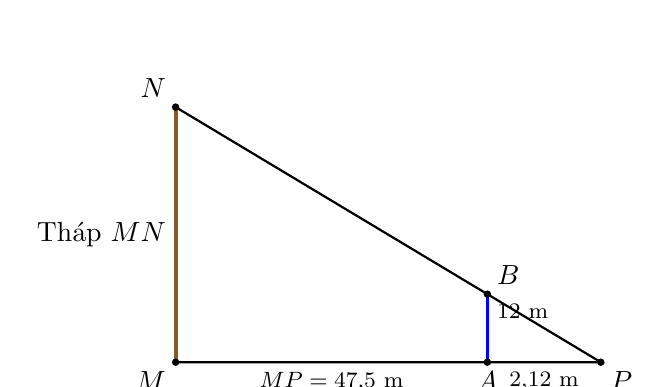
\begin{tikzpicture}[scale=0.9, >=stealth]
  \coordinate (M) at (0,0);
  \coordinate (N) at (0,3.6);
  \coordinate (P) at (6,0);
  \coordinate (A) at (4.4,0);
  \coordinate (B) at (4.4,0.96);
  \draw[thick] (M)--(P)--(N)--cycle;
  \draw[thick, blue] (A)--(B);
  \draw[line width=1.5pt, brown!70!black] (M)--(N);
  \fill (M) circle (1.5pt) node[below left] {$M$};
  \fill (N) circle (1.5pt) node[above left] {$N$};
  \fill (P) circle (1.5pt) node[below right] {$P$};
  \fill (A) circle (1.5pt) node[below] {$A$};
  \fill (B) circle (1.5pt) node[above right] {$B$};
  \node[left] at ($(M)!0.5!(N)$) {Tháp $MN$};
  \node[above right] at ($(A)!0.5!(B)$) {\footnotesize $12\text{ m}$};
  \node[below] at ($(A)!0.5!(P)$) {\footnotesize $2{,}12\text{ m}$};
  \node[below] at ($(M)!0.5!(A)$) {\footnotesize $MP = 47{,}5\text{ m}$};
\end{tikzpicture}
\end{center}
\begin{enumerate}[label=\textbf{\alph*)}, leftmargin=0.8cm, itemsep=2pt]
\item (0,75 điểm) Tính chiều cao $MN$ của tháp Bitexco.
\end{enumerate}
\end{ex}
\vspace{0.5mm}

\begin{ex} (0,5 điểm)
Chứng minh rằng $A = x^2 + 2xy + 4y^2 + 6y + 5 > 0$ với mọi $x, y$.
\begin{enumerate}[label=\textbf{\alph*)}, leftmargin=0.8cm, itemsep=2pt]
\item (0,5 điểm) Chứng minh $A > 0$ với mọi $x, y$.
\end{enumerate}
\end{ex}
\vspace{0.5mm}


\begin{center}
\rule{4cm}{0.4pt}\\
\textit{--- HẾT ---}
\end{center}
\end{document}
